\subsection{Pengujian Komponen \textit{Rule Manager}}

Pada bagian ini akan dijelaskan tentang tujuan, skenario, hasil, dan analisis dari pengujian komponen \textbf{\textit{Rule Manager}}.

\subsubsection{Tujuan Pengujian}

Tujuan pengujian ini memastikan komponen \textbf{\textit{Rule Manager}} dapat berjalan dengan baik dan menghasilkan data yang sesuai dengan ekspektasi.

\subsubsection{Skenario Pengujian}

\textbf{\textit{Rule Manager}} adalah komponen \textit{low-level} yang hanya akan digunakan oleh komponen lain. Sehingga, untuk melakukan pengujian ini, akan dilakukan dengan pendekatan pembuatan \textit{test driver} khusus. Pengujian terhadap komponen \textbf{\textit{Rule Manager}} dilakukan dengan beberapa skenario sebagai berikut.
\begin{enumerate}
    \item \bfseries Pembuatan \textit{Rule}\normalfont
    
        Skenario bertujuan untuk memastikan \textit{parser} bekerja secara benar dan menghasilkan \textit{rule} yang sesuai dengan ekspektasi. Diekspektasikan \textit{rule} terkait inisiasi, prosesor, dan memori berhasil di\textit{parse} dan program berjalan tanpa rusak serta parameter yang dimasukkan sesuai dengan data uji coba. 

    \item \bfseries Kebenaran \textit{Rule}\normalfont
    
        Skenario ditujukan untuk membuktikan bahwa \textit{rule} tetap berjalan pada kondisi simpleks maupun kompleks dan mengeluarkan \textit{output} yang sesuai saat di panggil.

    \item \bfseries Deklarasi Variabel dan Pengaksesan Variabel\normalfont
    
        Skenario mencakup fungsi \textit{rule} yang dapat mendeklarasikan variabel baru dan mengaksesnya pada \textit{rule} lain dan juga mengubahnya.
\end{enumerate}

\subsubsection{Hasil Pengujian dan Analisis}

% \begin{figure}[h]
%     \centering
%     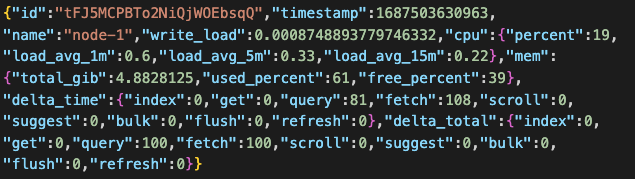
\includegraphics[width=0.8\textwidth]{chapter-4/mf-3.png}
%     \caption{Hasil Pengujian Komponen \textit{Metrics Fetcher} Skenario 3}
%     \label{fig:mf-3}
% \end{figure}

Pengujian komponen \textbf{\textit{Rule Manager}} sudah sesuai ekspektasi dan dapat dilanjutkan ke pengujian komponen lainnya.